\usetikzlibrary{circuits.ee.IEC}

\tikzset{circuit declare symbol = AC source}
\tikzset{AC source IEC graphic/.style={
    circuit symbol lines,
    circuit symbol size=width 2 height 2,
    shape=generic circle IEC,
    /pgf/generic circle IEC/before background={
    \pgfpathmoveto{\pgfpoint{-0.8pt}{0pt}}
    \pgfpathsine{\pgfpoint{0.4pt}{0.4pt}}
    \pgfpathcosine{\pgfpoint{0.4pt}{-0.4pt}}
    \pgfpathsine{\pgfpoint{0.4pt}{-0.4pt}}
    \pgfpathcosine{\pgfpoint{0.4pt}{0.4pt}}
    \pgfusepath{stroke}
    },
    transform shape, draw
  }
}
\tikzset{circuit ee IEC/.append style=
  {set AC source graphic = AC source IEC graphic}
}

\begin{figure}
    \centering
    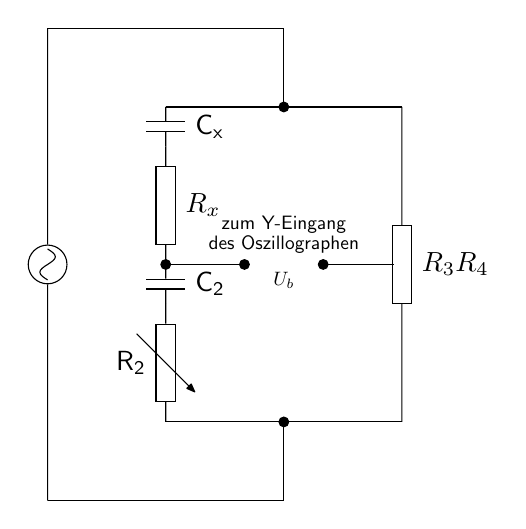
\begin{tikzpicture}[circuit ee IEC, font=\sffamily]
    \draw (0,0) to [AC source](0,-6);
    \draw (0,0) -- (3,0);
    \draw (3,0) -- (3, -1);
    \node[contact] at (3,-1) {};
    \draw (1.5, -1) -- (4.5, -1);
    \draw (1.5,-1) to [capacitor={info={C$\mathsf{_{x}}$},info'={$\mathsf{_{}}$}}] (1.5,-1.5);
    \draw (1.5, -1.5) to [resistor={info={$R_x$}}] (1.5, -3);
    \draw (1.5,-3) to [capacitor={info={C$\mathsf{_{2}}$},info'={$\mathsf{_{}}$}}] (1.5,-3.5);
    \draw (1.5, -3.5) to  [resistor={adjustable={info={$\mathsf{_{}}$}}, info'={R$\mathsf{_{2}}$}}] (1.5,-5);
    \draw (4.5, -1) to [resistor={info={$R_3$ \\ $R_4$}}] (4.5, -5);
    \node[scale=0.7] at (3, -2.5) {zum Y-Eingang};
    \node[scale=0.7] at (3,-2.75) {des Oszillographen};
    \node[scale=0.7] at (3,-3.2) {$U_b$};
    \node[contact] at (1.5,-3) {};
    \node[contact] at (2.5, -3) {};
    \node[contact] at (3.5,-3) {};
    \draw (1.5, -3) -- (2.5, -3);
    \draw (3.5, -3) -- (4.4, -3);
    \draw (1.5, -5) -- (4.5, -5);
    \node[contact] at (3,-5) {};
    \draw (0, -6) -- (3,-6);
    \draw (3, -6) -- (3,-5);
    \end{tikzpicture}
    \caption{Kapazitätsmessbrücke}
    % \label{fig:Kapazitätsmessbrücke}
\end{figure}
